%--------------------------------------------------------------------
%--------------------------------------------------------------------
% Formato para los talleres del curso de Métodos Computacionales
% Universidad de los Andes
%--------------------------------------------------------------------
%--------------------------------------------------------------------

\documentclass[11pt,letterpaper]{exam}
\usepackage[utf8]{inputenc}
\usepackage[spanish]{babel}
\usepackage{graphicx}
\usepackage{tabularx}
\usepackage[absolute]{textpos} % Para poner una imagen en posiciones arbitrarias
\usepackage{multirow}
\usepackage{float}
\usepackage{hyperref}
%\decimalpoint

\begin{document}
\begin{center}
{\Large Métodos Computacionales} \\
\textsc{Tarea 2}\\
01-2019\\
\end{center}

\noindent
\section{Ejercicio 2: Fourier}
\begin{center}
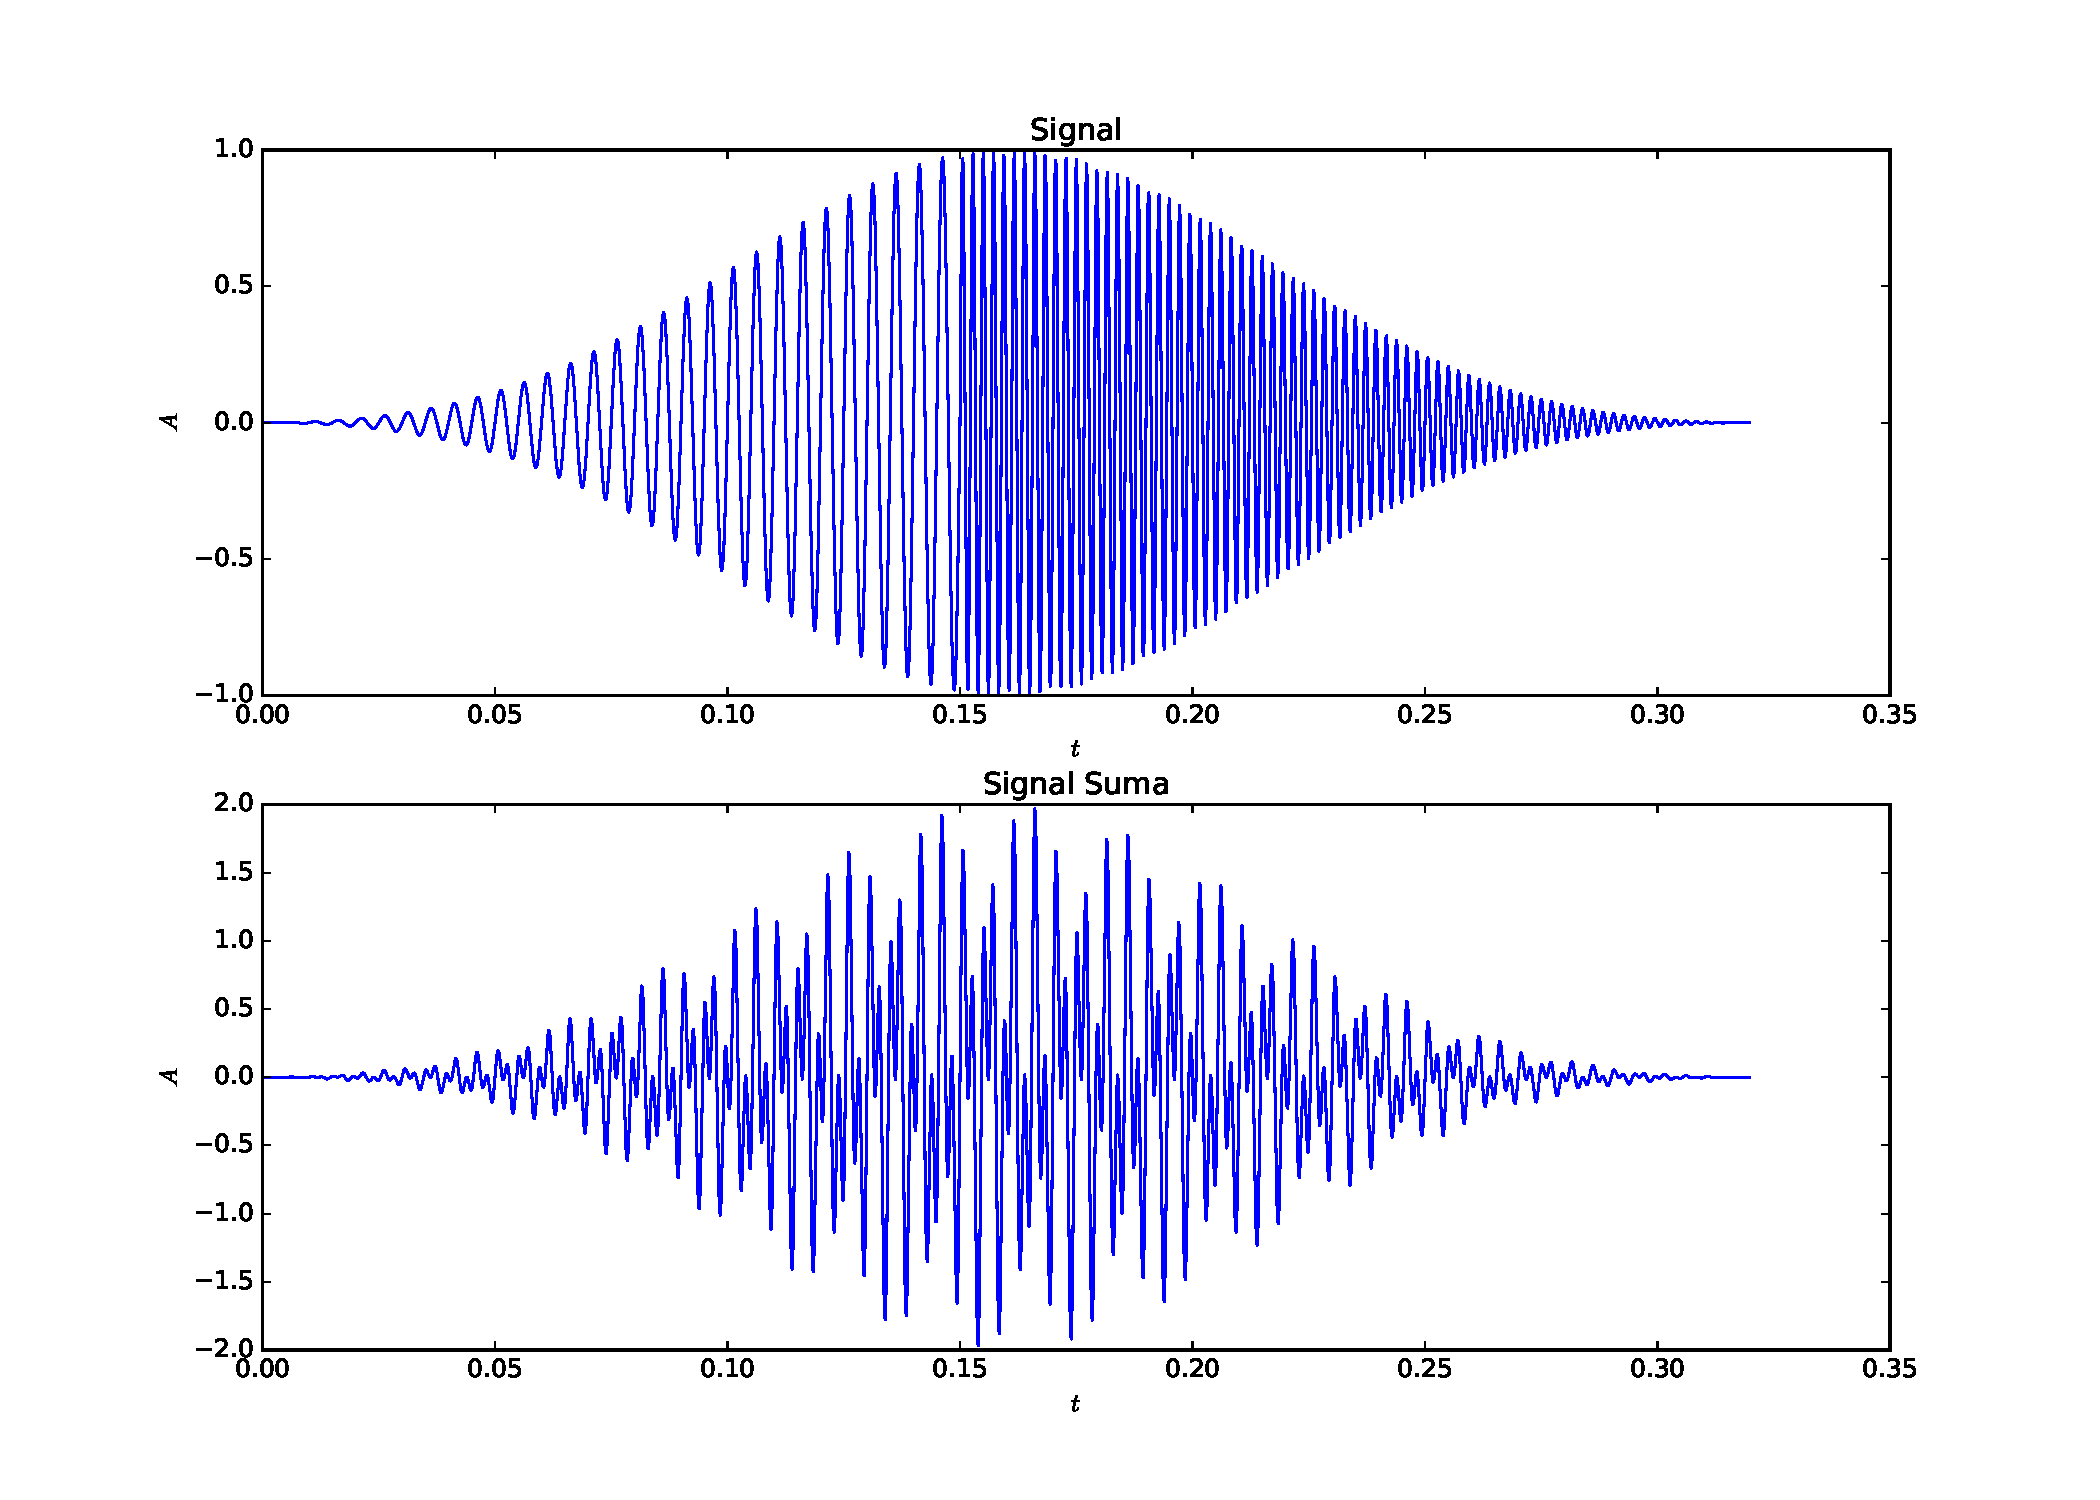
\includegraphics[width=10cm]{2_Signal.pdf} 
\begin{center}
\begin{center}
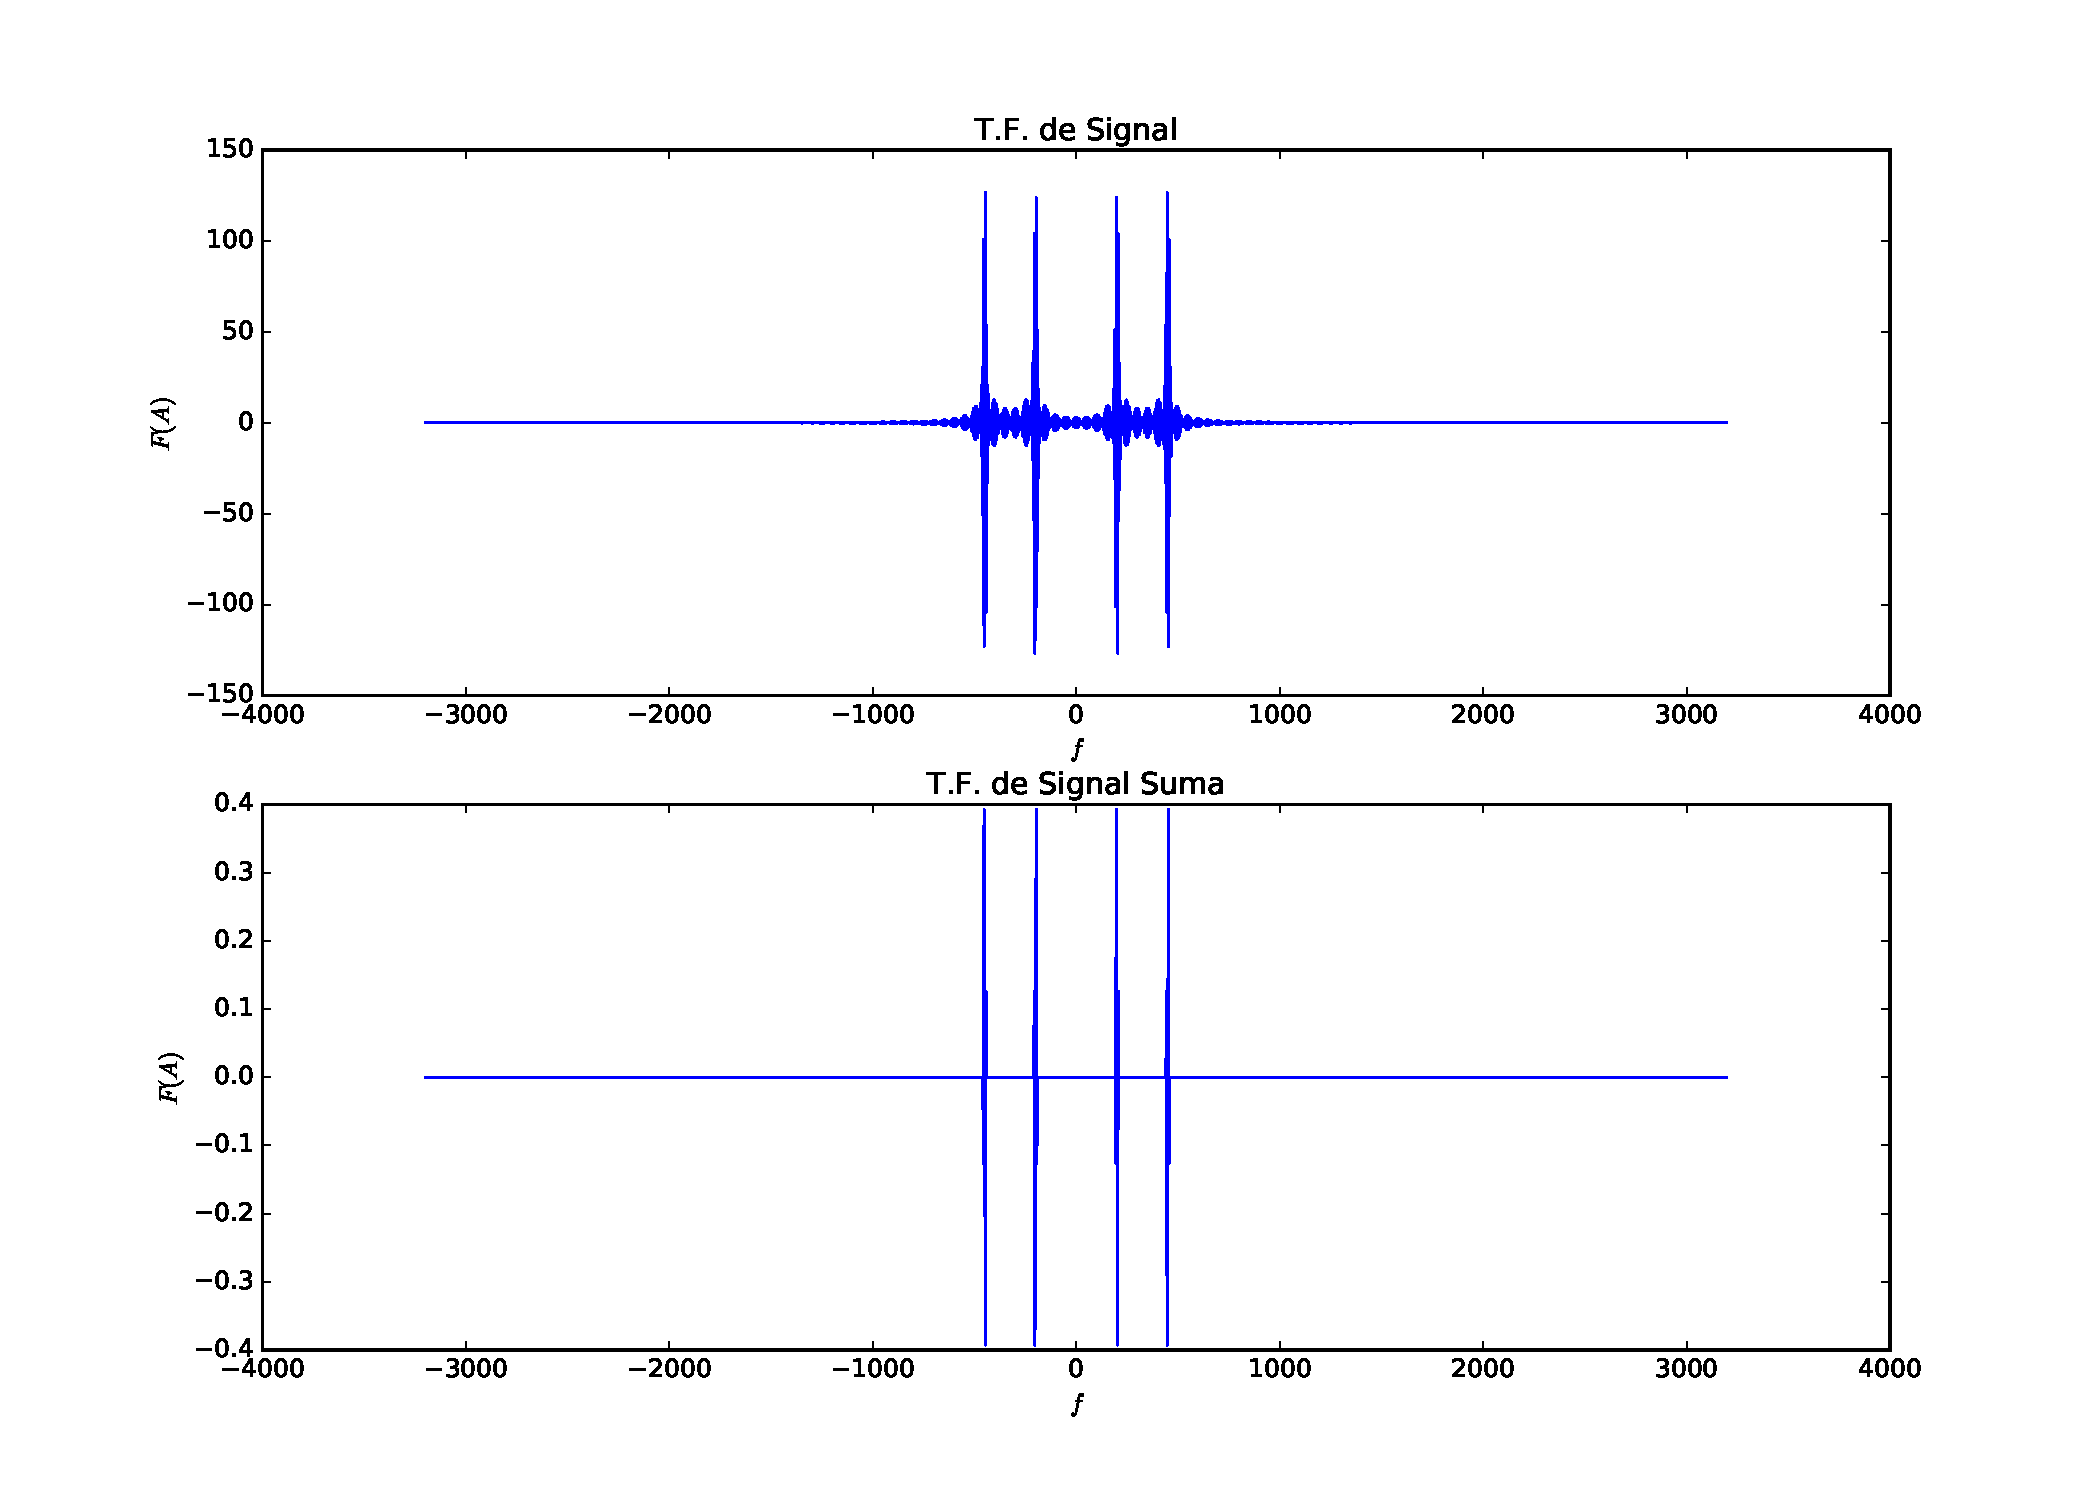
\includegraphics[width=10cm]{2_FourierSignal.pdf} 
\begin{center}
\begin{center}
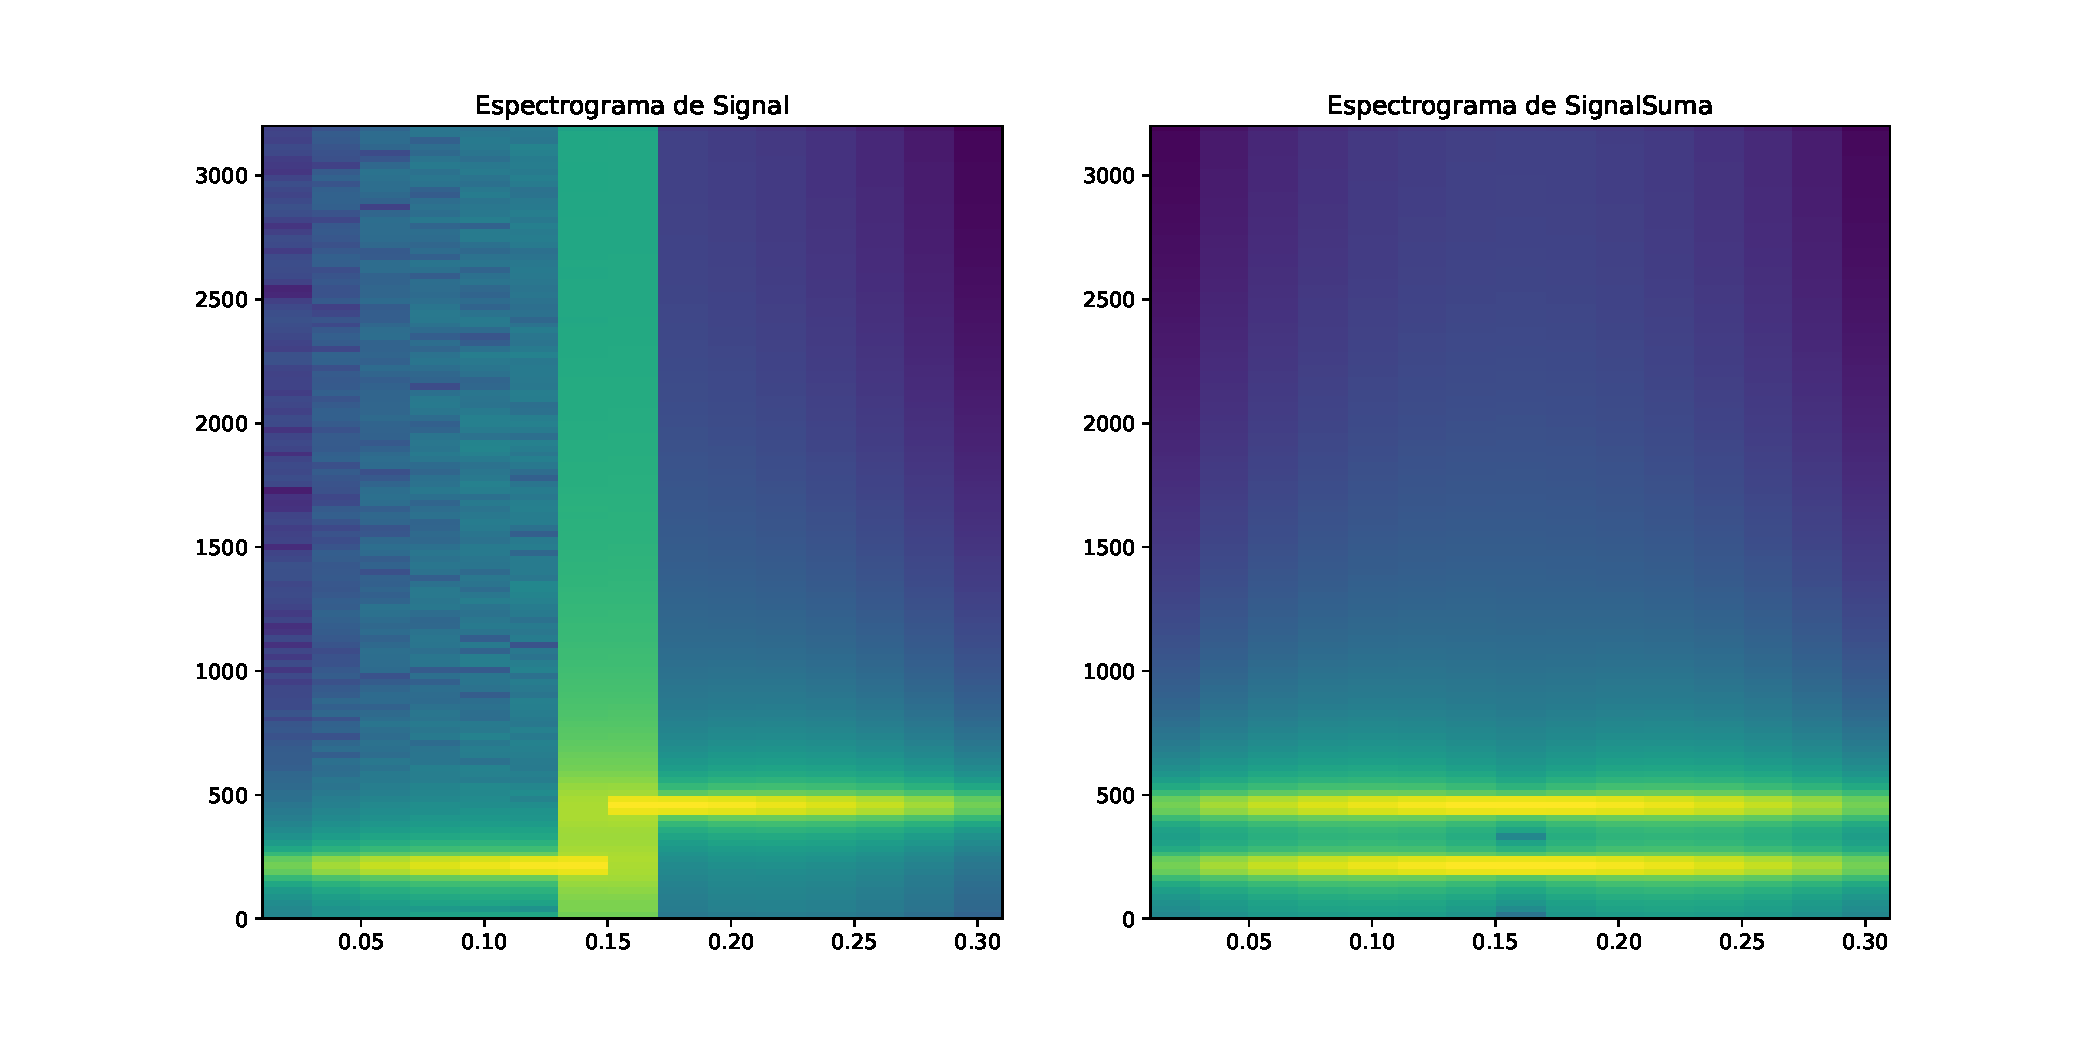
\includegraphics[width=10cm]{2_Espectrogramas.pdf} 
\begin{center}

%Analisis de resultados...

\end{document}
